\documentclass[tikz,border=10pt]{standalone}
\usepackage{tikz}
\usetikzlibrary{shapes,arrows,positioning,fit,backgrounds}

\begin{document}
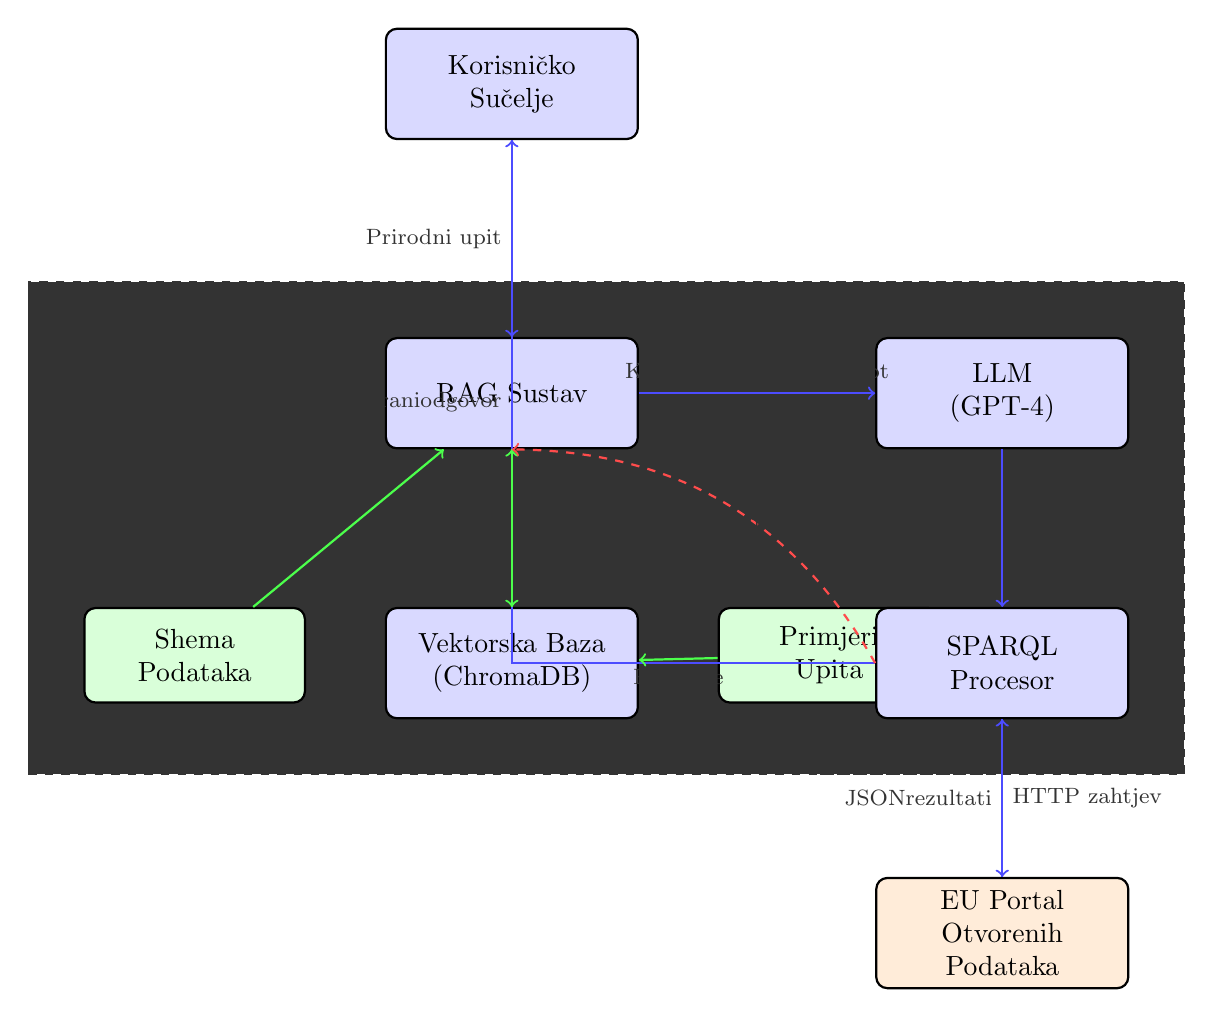
\begin{tikzpicture}[
    node distance=2cm,
    box/.style={rectangle, draw, rounded corners, minimum width=2.5cm, minimum height=1cm, align=center},
    component/.style={rectangle, draw, rounded corners, minimum width=3.2cm, minimum height=1.4cm, align=center, fill=blue!15, thick},
    data/.style={rectangle, draw, rounded corners, minimum width=2.8cm, minimum height=1.2cm, align=center, fill=green!15, thick},
    external/.style={rectangle, draw, rounded corners, minimum width=3.2cm, minimum height=1.4cm, align=center, fill=orange!15, thick},
    arrow/.style={->, thick, color=blue!70},
    data_arrow/.style={->, thick, color=green!70},
    feedback_arrow/.style={->, thick, color=red!70, dashed},
    label/.style={font=\footnotesize, color=black!80}
]

% Top row - User Interface
\node[component] (user) {Korisničko\\Sučelje};

% Middle row - Core processing
\node[component, below=2.5cm of user] (rag) {RAG Sustav};
\node[component, right=3cm of rag] (llm) {LLM\\(GPT-4)};

% Bottom row - Data and services
\node[data, below left=2cm and 1cm of rag] (schema) {Shema\\Podataka};
\node[component, below=2cm of rag] (vector) {Vektorska Baza\\(ChromaDB)};
\node[data, below right=2cm and 1cm of rag] (examples) {Primjeri\\Upita};

\node[component, below=2cm of llm] (sparql) {SPARQL\\Procesor};
\node[external, below=2cm of sparql] (euportal) {EU Portal\\Otvorenih\\Podataka};

% Background grouping boxes
\begin{scope}[on background layer]
    \node[fit=(rag)(vector)(examples)(schema), draw, dashed, inner sep=0.7cm, 
          fill=blue!5, label={[font=\small]above:Obrada i Pretraga}] {};
    \node[fit=(llm)(sparql), draw, dashed, inner sep=0.7cm, 
          fill=yellow!5, label={[font=\small]above:Generiranje i Izvršavanje}] {};
\end{scope}

% Main flow arrows
\draw[arrow] (user) -- node[label, left] {Prirodni upit} (rag);
\draw[arrow] (rag) -- node[label, above] {Kontekstualizirani\\prompt} (llm);
\draw[arrow] (llm) -- node[label, right] {SPARQL\\upit} (sparql);
\draw[arrow] (sparql) -- node[label, right] {HTTP zahtjev} (euportal);
\draw[arrow] (euportal) -- node[label, left] {JSON\\rezultati} (sparql);
\draw[arrow] (sparql) -| node[label, near end, left] {Formatirani\\odgovor} (user);

% Data flow arrows
\draw[data_arrow] (rag) -- node[label, left] {Semantička\\pretraga} (vector);
\draw[data_arrow] (vector) -- node[label, right] {Slični\\primjeri} (rag);
\draw[data_arrow] (examples) -- node[label, below] {Punjenje} (vector);
\draw[data_arrow] (schema) -- node[label, above left] {Metadata} (rag);

% Feedback loop
\draw[feedback_arrow, bend right=30] (sparql.west) to node[label, below] {Validacija grešaka} (rag.south);

\end{tikzpicture}
\end{document}